\documentclass[tikz,border=4pt]{standalone}
% Estilo común de los diagramas de bloques (se usa con \input en cada standalone)
\usepackage[defaultsans,scale=0.92]{lato}
\usepackage{libertinust1math}
\usepackage{xcolor,amsmath}
\usepackage{tikz}
\usetikzlibrary{positioning,arrows.meta,calc,shapes.geometric}
\usepackage{../../notacion}
\definecolor{ctrlazul}{HTML}{1E5AA8}\definecolor{ctrlnoche}{HTML}{14213D}
\definecolor{ctrlcoral}{HTML}{D1495B}\definecolor{ctrlverde}{HTML}{2A9D8F}
\definecolor{ctrlambar}{HTML}{E09F3E}\definecolor{ctrlgris}{HTML}{5C677D}
\definecolor{ctrlvioleta}{HTML}{6C4AB6}\definecolor{ctrlteal}{HTML}{0F7173}
\tikzset{
  >={Stealth[length=2.4mm]}, every node/.style={font=\small},
  bloque/.style={draw=ctrlnoche,fill=ctrlazul!7,thick,rounded corners=1.5pt,minimum height=9mm,minimum width=13mm,inner sep=4pt},
  suma/.style={draw=ctrlnoche,thick,circle,inner sep=0pt,minimum size=6mm},
  senal/.style={->,thick,draw=ctrlnoche},
  rot/.style={font=\footnotesize,text=ctrlgris},
}

\begin{document}
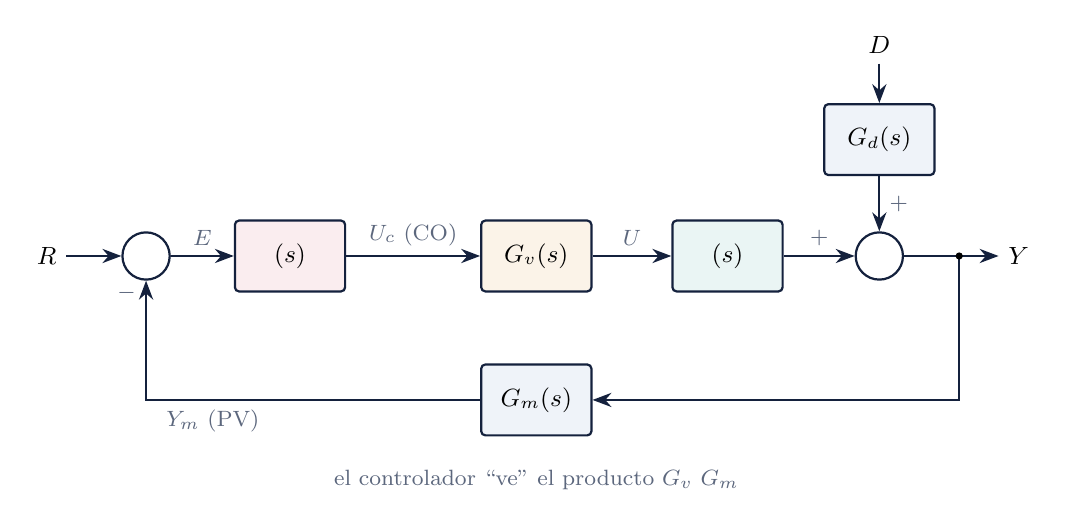
\begin{tikzpicture}[b/.style={bloque,minimum width=14mm}]
  \node (r) {$R$};
  \node[suma,right=7mm of r] (S) {};
  \node[b,right=8mm of S,fill=ctrlcoral!10] (c) {$\Gc(s)$};
  \node[b,right=17mm of c,fill=ctrlambar!12] (v) {$G_v(s)$};
  \node[b,right=10mm of v,fill=ctrlverde!10] (p) {$\Gp(s)$};
  \node[suma,right=9mm of p] (S2) {};
  \node[b,above=7mm of S2] (d) {$G_d(s)$};
  \node[above=5mm of d] (D) {$D$};
  \coordinate[right=7mm of S2] (o); \node[right=5mm of o] (y) {$Y$};
  \node[b,below=9mm of v] (m) {$G_m(s)$};
  \draw[senal] (r)--(S);
  \draw[senal] (S)--node[above,rot]{$E$}(c);
  \draw[senal] (c)--node[above,rot]{$U_c$ (CO)}(v);
  \draw[senal] (v)--node[above,rot]{$U$}(p);
  \draw[senal] (p)--node[above,rot]{$+$}(S2);
  \draw[senal] (D)--(d); \draw[senal] (d)--node[right,rot]{$+$}(S2);
  \draw[thick,draw=ctrlnoche] (S2)--(o); \draw[senal] (o)--(y);
  \draw[senal] (o)|-(m);
  \draw[senal] (m)-|node[pos=0.95,left,rot]{$-$}node[pos=0.4,below,rot]{$Y_m$ (PV)}(S);
  \fill (o) circle (1.3pt);
  \node[rot,below=3mm of m] {el controlador ``ve'' el producto $G_v\,\Gp\,G_m$}; 
\end{tikzpicture}
\end{document}
